\section{Test di ipotesi}\linkdest{test}

\subsection{Ipotesi semplici}

\begin{frame}{Testing simple hypothesis}

\begin{block}{Test: funzione dallo spazio delle osservabili in H.}
	Un'ipotesi \'e un'affermazione sui parametri che caratterizzano lo stato della natura; se l'ipotesi non \'e sufficienta a determinare distribuzione di probabilit\'a della nostra osservabile l'ipotesi \'e composta: se ipotesi da falsificare \'e non esistenza higgs ($m=0$) semplice, ma alternativa \'e composta da $m>0$
\end{block}
\begin{block}{Choosing a test for $H_0$ amount to choosing test statistic and critical region}
\end{block}
\begin{block}{Regione critica(C)/di accettazione($\overline{C}$) nello spazio delle X}
	Due sottoinsiemi di X individuano la regione critica e regione di accettazione (conferma $H_0$).
\end{block}
\begin{block}{GOF: test $H_0$ vs not $H_0$}
\end{block}
\end{frame}

\begin{frame}{Propriet\'a dei test. MP test.}
\begin{block}{errore tipo I/II}
\begin{itemize}
	\item Errore di tipo I (falso positivo), scarto $H_0$ quando \'e vera (loss,size,taglia,livello di significativit\'a $\alpha=\prob{(x\in C|H_0)}=\prob_0{(x\in C)}$.
	\item Errore tipo II (falso negativo, contaminazione): probabilit\'a di accettare erroneamente $H_0$, $\prob{(x\in\overline{C}|\not{H_0})}=\beta$. Potenza del test $1-\beta=\prob{(x\in C|H_1)}$ \'e la capacit\'a di distinguere ipotesi diverse da $H_0$ 
\end{itemize}
\end{block}
\end{frame}

\begin{frame}{Comparison of tests: power}
Ipotesi semplici: $H_0: \theta=\theta_0$, $H_1: \theta=\theta_1$. Power $1-\beta=p(\theta_1)$.
Ipotesi composte: $p(\theta)=1-\beta(\theta)$.
\begin{figure}[!ht]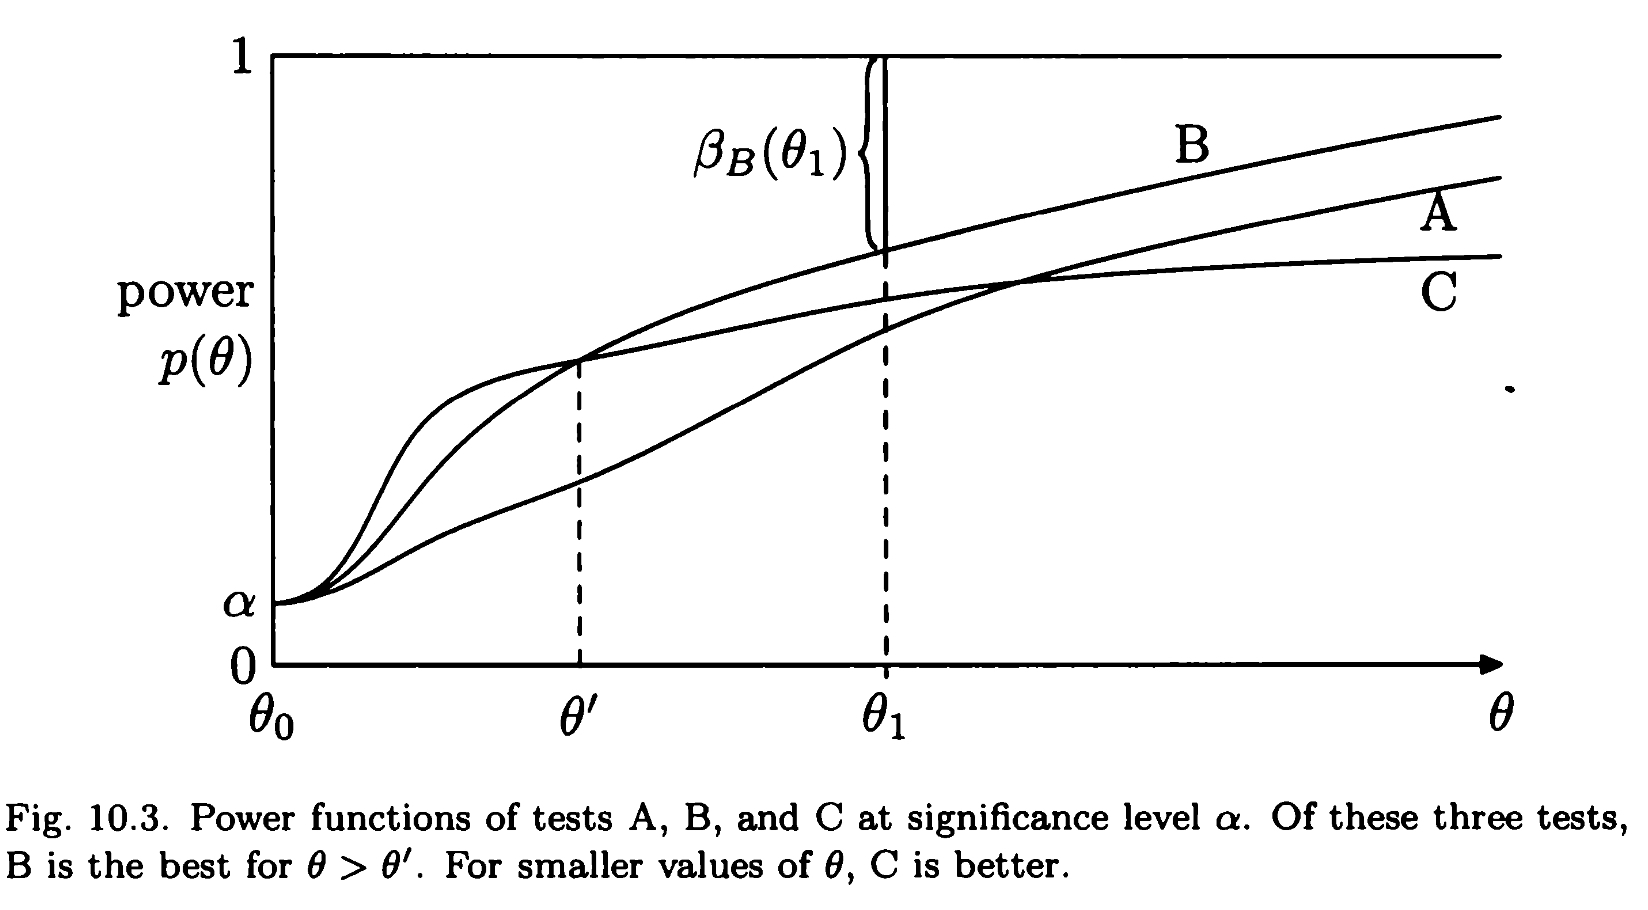
\includegraphics[trim={0cm 0cm 0 0},clip, keepaspectratio,width=0.5\textwidth]{mostpower}\label{fig:mostpower}\end{figure}

\begin{block}{Ottimizzazione: power maggiore possibile.}
	UMP test: power maggiore uguale a qualunque test per tutte le ipotesi: esiste?
\end{block}
\end{frame}

\begin{frame}{Consistenza e bias}
\begin{block}{Propriet\'a dei test}
	\begin{itemize}
		\item Consistenza: $\lim_{N\to\infty}\prob{(\vec{X}\in w_{\alpha}|H_1)}=1$ non \'e detto che sia uniforme.
		\item unbiasedness $\pow{}=1-\beta\geq\alpha, \forall i$, T consistente \'e asintoticamente unbiased.
	\end{itemize}
\end{block}
\begin{figure}[!ht] \begin{subfigure}[b]{0.47\textwidth} \centering 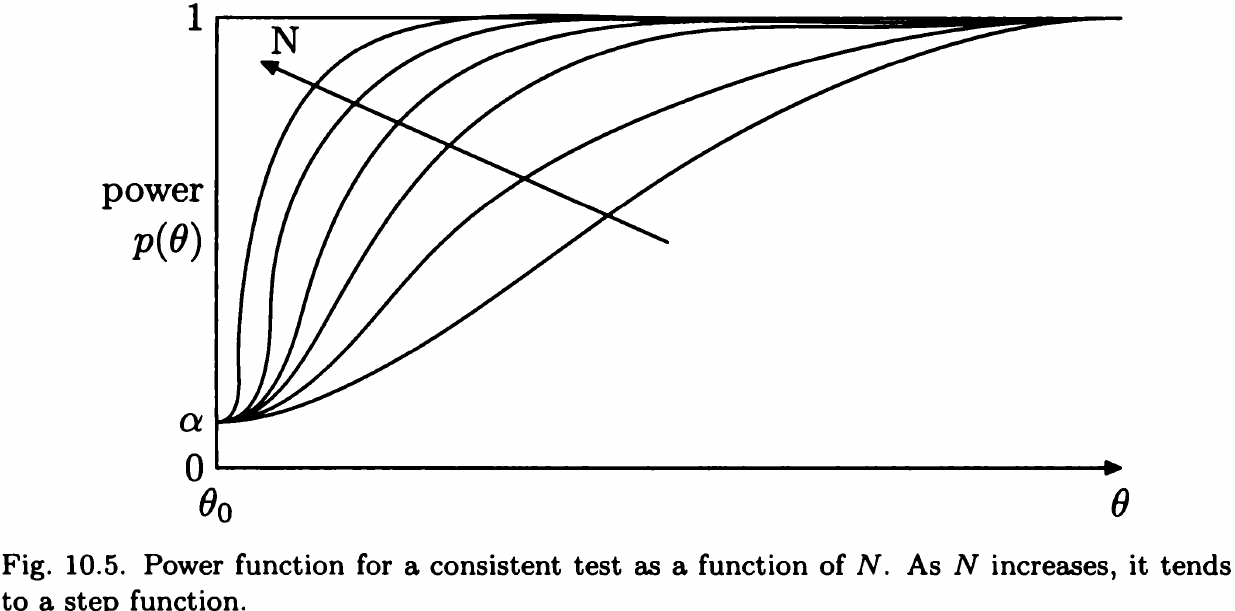
\includegraphics[trim={0cm 0 0 0},clip, width=0.99\textwidth]{powerconsistent} \label{fig:powerconsistent} \end{subfigure} ~ \begin{subfigure}[b]{0.47\textwidth} \centering 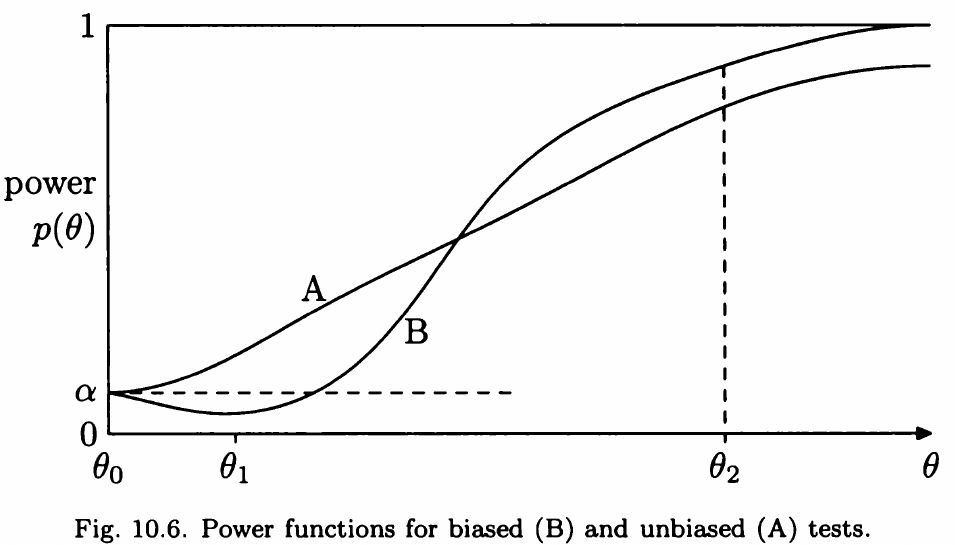
\includegraphics[trim={0cm 0 0 0},clip,width=0.99\textwidth]{biasedtest}\label{fig:biasedtest}\end{subfigure} \end{figure} 
Test B can't distinguish between $\theta_0$, $\theta_1$.
\end{frame}

\begin{frame}{Symmetry between $\alpha$ and $\beta$}
Unrealistic in experimental situation to keep $\alpha$ constant:$\alpha=p(\theta_0)$ $\beta=p(\theta_1)$ as function of $\alpha$, dotted line $\alpha=1-\beta$ below which tests are unbiased
\begin{figure}[!ht]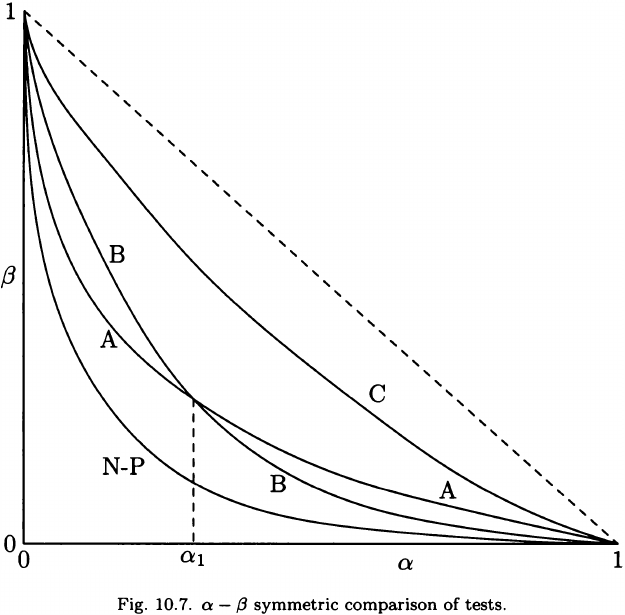
\includegraphics[trim={0cm 0cm 0 0},clip, keepaspectratio,width=0.5\textwidth]{testabsym}\label{fig:testabsym}\end{figure}
\end{frame}

\begin{frame}{Lemma di Neyman-Pearson (Test di NP)}\frameintoc
\begin{block}{Statistica di un test}
Posso esprimere un test in funzione di una statistica: $T(\vec{x})=T(t(\vec{x}))$ (nel caso del lemma NP la statistica \'e il LR). 
\end{block}
\begin{block}{Test NP}
%Lo spazio dei parametri \'e costituito da $\theta_0$, $\theta_1$: l'MP test \'e quello che mi da come regione critica gli x tali che $\frac{\prob_0{(x)}}{\prob_1{(x)}}<q(\alpha)$, $q$ \'e determinato da condizione $\prob{(C|H_0)}\leq\alpha$ (LR), questo \'e il test di massimo power.
RV $\vec{X}$: pdf $f_N(\vec{X}|\theta)$, lo spazio dei parametri \'e $\theta_0,\theta_1$. Cerco la regione $w_{\alpha}$ che massimizza power $1-\beta$ (dato $\alpha$):
\begin{align*}
&\int_{w_{\alpha}}f_N(\vec{X}|\theta_0)\,dX=\alpha(1-\alpha)\\
&\int_{w_{\alpha}}f_N(\vec{X}|\theta_1)\,dX=1-\beta\\
&=\int_{w_{\alpha}}\frac{f_N(\vec{X}|\theta_1)}{f_N(\vec{X}|\theta_0)}f_N(\vec{X}|\theta_0)\,dX=\E_{w_{\alpha}}{[\frac{f_N(\vec{X}|\theta_1)}{f_N(\vec{X}|\theta_0)}|\theta_0]}\\
&\Rightarrow l_N(\vec{X},\theta_0,\theta_1)=\frac{f_N(\vec{X}|\theta_1)}{f_N(\vec{X}|\theta_0)}\geq c_{\alpha}: H_1\ (\leq c_{\alpha}: H_0)
\end{align*}
scelto in maniera che il livello di confidenza sia $\alpha(1-\alpha)$
\end{block}
\end{frame}

\begin{wordonframe}{Dimostrazione lemma Neyman-Pearson}
Per ogni test alternativo $T'$ prendo $\alpha'\leq\alpha_{NP}$ allora $\beta'\geq\beta_{NP}$ ($\pow'\leq\pow_{NP}$, probabilit\'a errore tipo II \'e maggiore), dimostro $\beta'-\beta\geq0$ cio\'e $\prob{(\overline{C}'|H_1)}-\prob{(\overline{C}|H_1)}$:
\begin{align*}
&\prob{(C|H_1)}-\prob{(C'|H_1)}=\prob{(C\cap|H_1)}+\prob{(C\cap\overline{C}'|H_1)}-\prob{(C\cap C'|H_1)}-\prob{(C'\cap\overline{C}|H_1)}=\prob{(C\cap\overline{C}'|H_1)}-\prob{(C'\cap\overline{C}|H_1)}\\
&\prob{(C\cap C'|H_1)}=\int_{C\cap C'}\prob_1{(x)}\,dx\geq\int_{C\cap \overline{C}'}\frac{\prob_0{(x)}}{q}\,dx=\frac{1}{q}\prob{(C\cap\overline{C}'|H_0)}
\end{align*}
\end{wordonframe}

\subsection{Ipotesi composte}

\begin{frame}{Ipotesi composte}
One family pdf $f(\vec{X},\theta)$: $H_0$ per $\theta<\theta_0$, $H_1$ per $\theta>\theta_1$
\end{frame}

\begin{frame}{Test UMP unilaterale per famiglia esponenziale: Karlin-Rubin theorem.}
$X_1,\ldots,X_N$ N iid: pdf della forma $\prob{(x,\mu)}=F(x)G(\mu)\Exp{[A(x)B(\mu)]}$ e $B(\mu)$ (monotona):

UMP test (one-sided) per distinguere $H_0: \mu\leq\mu_0$, $H_{\mu}: \mu>\mu_0$; applico NP per $\mu_0$ e $\mu$, MP test ha la forma

\[\frac{F^N(x)G^N(\overline{\mu})}{F^N(x)G^N(\overline{\mu}_0)}\Exp{[\sum_iA(x_i)](B(\overline{\mu})-B(\overline{\mu}_0))}\gtrless c_{\alpha}\]
$F,G>0$.
Se il likelihood ratio \'e funzione monotona di una statistica $T(\vec{X})=\sum_iA(x_i)$ e scelgo $\alpha$ e $k_{\alpha}$ tali che $\prob{[\lr{(T(x))}\geq c_{\alpha}]}=\alpha$  allora la regione critica per un test UMP unilaterale $H_0$ vs $H_1$ \'e $C=\{x:T(x)\geq k_{\alpha}\}$.

\cite[5]{lrtmptumpt}; \cite[445]{inferencemukhopadhyay2000}; \cite[sec 3.6]{lehmann2006testing}
\end{frame}

\begin{frame}{Test UMP parametro non contenuto nell'intervallo vs contenuto (ma non viceversa)}

\cite[269]{james2006statistical}\cite[sec 3.7]{lehmann2006testing}
\end{frame}

\begin{wordonframe}{One/two-sided test}
%insert-fig 10.9: oneone2sides
$1+$ \'e il power per UMP test per $\theta>\theta_0$, $1-$ \'e il power per UMP test per $\theta<\theta_0$: if the size of one sided tests is $\frac{\alpha}{2}$ that of two-sided (sum of the two one-sided) is $\alpha$
\end{wordonframe}

\begin{frame}{Local most powerfull (LMP) tests}
(LMP) Se ho bisogno di massima sensibilit\'a vicino alla soglia: $1-\beta$ grande nelle vicinanze di 0: $H_0$: $\theta=\theta_0$, $H_1$: $\theta=\theta_0+\Delta$, quindi $\ln{L(\vec{X},\theta_1)}\approx\ln{L(\vec{X},\theta_0)}+\Delta\PDy{\theta}{\ln{L}}|_{\theta_0}$.
Applico NP a $H_0$ vs $H_1$:
\begin{align*}
&\ln{L(\vec{X},\theta_1)}-\ln{L(\vec{X},\theta_0)}\gtrless c_{\alpha} \Rightarrow \PDy{\theta}{\ln{L}}\gtrless q_{\alpha}\\
&\E{[\PDy{\theta}{\ln{L}}|_{\theta_0}]}=0,\ \E{[(\PDy{\theta}{\ln{L}})^2]}=NI
\end{align*}

score \'e asintoticamente normale Test: $\PDy{\theta}{\ln{L}}|_{\theta_0}\gtrless\lambda_{\alpha}\sqrt{NI}$.
\end{frame}

\begin{frame}{Likelihood ratio test (LRT)}\frameintoc
Sia $H_0: \vec{\theta}\in\nu$, $H_0: \vec{\theta}\in\overline{\nu}$
\begin{block}{test statistic maximum likelihood ratio}
 $\lambda=\frac{\max_{\vec{\theta}\in\nu}L(\vec{X},\theta)}{\max_{\vec{\theta}\in\overline{\nu}}L(\vec{X},\theta)}$
\end{block}
\begin{block}{critical region, significance level and power for continuus families of Hypotheses}
$\alpha=\sup{\prob{(\lambda(\vec{X})\leq k;\theta\in\theta_0)}}$.
Se $H_0$ impone r vincoli sugli $r+s$ parametri di $H_0, H_1$: $\forall\theta\in H_0$ $-2\log{\lambda}\to\chi^2_{r}$, $\forall\theta\in H_1$ $-2\log{\lambda}\to\chi^2_{r}$ non centrale con parametro $K_1=(\vec{\theta}_r-\vec{\theta}_{r0})^TI_r(\vec{\theta}_r-\vec{\theta}_{r0})$.
Regione critica: $-2\ln{\lambda}>\chi^2_{\alpha}(r)$, power:
\begin{equation*}
p=1-\beta=\int_{\chi_{\alpha}^2(r)}^{\infty}dF_1[\chi^2(r,K_1)]\approx\int_{(\frac{r+K_1}{r+2K_1})\chi^2_{\alpha}(r)}^{\infty}dF_2[\chi^2(r+\frac{K_1^2}{r+2K_1})]
\end{equation*}
\end{block}

\end{frame}

\begin{wordonframe}{LRT: }
\begin{block}{Espansione in $\hat{\theta}-\theta_0$ per $\theta=\theta_0$}
	Usually the critical region is determined via asymptotic pdf of LR:
	$l(\theta_0)=-\log{L}=l(\hat{\theta})+\frac{1}{2}l''(\hat{\theta})(\hat{\theta}-\theta_0)^2$ $L(\vec{X}|\vec{\theta})\propto\exp{-\frac{1}{2}\E{(\PtwoDy{\theta}{\ln{L}})}(\hat{\theta}-\theta)^2}=\exp{-\frac{1}{2}(\hat{\theta}-\theta)^TI(\hat{\theta}-\theta)}$ (pdf asintoticamente normale con matrice covarianza $\invers{I}$). Quindi $I(\theta_0)(\hat{\theta}-\theta)^2\xrightarrow{D}\chi_1^2$.
\end{block}
\begin{block}{Asymptotic properties of MLE}

\end{block}
\end{wordonframe}

\begin{wordonframe}{Test of some theories with different dof}
%insert-fig 10.10
Maximum likelihood ratio for A vs generale case: $\lambda_a=\frac{L(0)}{L(d)}$, if hypothesis A is true $-2\ln{\lambda_a}$ is distributed asymptotically as $\chi^2(2)$; to test B vs general case ml ratio is $-2\ln{\lambda_a}$, distributed asymptotically as $\chi^2(1)$.
\end{wordonframe}

\begin{wordonframe}{Is data normally distributed (unknown variance)}
$X_1,,X_N$ iid $N(\mu,\sigma^2)$, $H_0: \mu=0,\sigma^2$, $H_1: \mu\neq0,\sigma^2$. Likelihood function is: 
\begin{equation*}
L(\mu,\sigma^2)=\frac{1}{(2\pi)\expy{N/2}\sigma^N}\exp{-\frac{1}{2}\sum^N\frac{(X_i-\mu)^2}{\sigma^2}}
\end{equation*}
Maximum likelihood estimators:
\begin{align*}
&H_0: \hat{\sigma}^2=\frac{1}{N}\sum_iX_i^2\\
&\max_{\sigma^2}L(0,\sigma)=\frac{\exp{-N/2}}{(2\pi)\expy{N/2}(\sum_iX_i/N)\expy{N/2}}\\
&H_1: \hat{\mu}=\exv{X},\ S^2=\frac{1}{N}\sum^N(X_i-\exv{X})^2\\
&\max_{\sigma^2}L(0,\sigma)=\frac{\exp{-N/2}}{(2\pi)\expy{N/2}(\sum_i(X_i-\exv{X})^2/N)\expy{N/2}}\\
\end{align*}
Likelihood ratio:
\begin{align*}
&\lambda=(\frac{\sum^N(X_i-\exv{X})^2}{\sum_iX_i^2})\expy{N/2}\\
&\lambda\expy{2/N}=\frac{1}{1+\frac{t^2}{N-1}}\\
&t=\frac{\sqrt{N}\exv{X}}{\sqrt{\frac{1}{N-1}}\sum(X_i-\exv{X})^2}=\sqrt{N}\frac{\exv{X}}{s}
\end{align*}
Test based on $\lambda$ is equivalent to test based on two-sided t-test: the critical region correspond to small $\lambda$.
\end{wordonframe}

\begin{wordonframe}{Test whether Poissonian data have same mean}
$X_1,,X_n$ iid RV poissonian with mean $\mu_i$. $H_0: \mu_1=\mu_2=\ldots=\mu$, $H_1: \mu_i$; MLE and likelihood ratio:
\begin{align*}
&L(\mu_1,\ldots,\mu_N)=\prod_i\exp{-\mu_i}\frac{\mu_i^{X_i}}{X_i!}\\
&H_0: \hat{\mu}=\exv{X},\ \max_{\mu}L(\mu)=\frac{\exp{N\exv{X}}\exv{X}\expy{N\exv{X}}}{\prod_iX_i!}\\
&H_1: \hat{\mu}_i=X_i,\ \max_{\mu_i}L(\mu_1,\ldots,\mu_N)=\exp{N\exv{X}}\exv{X}\expy{N\exv{X}}\prod_iX_i\expy{X_i}/X_i!\\
&\lambda=\frac{\exv{X}\expy{N\exv{X}}}{\prod_iX_i\expy{X_i}}
\end{align*}
Si ritrova la statistica $\sum_i^N(X_i-\exv{X})^2/\exv{X}$ (asintotic. come $\chi^2(N-1)$) considerando $X_i=\exv{X}+\delta_i$:
\begin{align*}
&\ln{\lambda}=N\exv{X}\ln{\exv{X}}-\sum_i(\exv{X}+\delta_i)\ln{\exv{X}}-\sum_i(\exv{X}+\delta_i)(\frac{\delta_i}{\exv{X}}\\
&-\frac{\delta_i^2}{2\exv{X}^2}+\ldots)
\end{align*}
\end{wordonframe}

\begin{wordonframe}{Max power test in intervallo}
	\begin{itemize}
		\item \'E possible espansione L in intervallo?
		\item Metodo empirico del LR. Uso stimatore ML $\hat{\mu}$: $t_{NP}=\frac{L(H_0)}{L(H_{\mu})}$. Introduco $\lambda=2\log{\frac{\sup_{\mu}}{L(\mu_0)}}$; Ipotesi complesse: $H_0: p(x;\mu_0,\nu)$ $H_{\mu}: p(x;\mu,\nu)$, $\prob{(\lambda)}\to \chi^2_{\dim{\mu-\nu}}$
	\end{itemize}
\end{wordonframe}

\subsection{esempi di test}

\begin{wordonframe}{Power}
	plot power(i) parte da $\alpha$ e va a 1 al crescere di i (separazione ipotesi) e pi\'u rapidamente al crescer di N.
	il grafico del power ($\prob{(\text{reject} H_0)| H_i}$) in funzione dell'indice i che identifica le ipotesi (per $H_0$ fa $\beta=1-\alpha$ quindi il power \'e $\alpha$) allontanandosi da $H_0$ deve essere il pi\'u grande possibile. 
\begin{block}{grafico $\prob_0{(X)}$ vs $\prob_1{(X)}$ con definizione di regione critica}
	\begin{picture}(100,130)
	\put(20,20){
		\begin{tikzpicture}[scale=0.3]
		\begin{axis}[title={Regione critica/accettanza per $H_0$},name=testh0,samples=100,ymin=0,xmin=0,xmax=10,xlabel={$x$},ylabel={$\prob{(x)}$},extra x ticks={1.3},extra x tick style={% changes for extra x ticks
			tick label style={yshift=-4mm}},
		]
		\addplot[id=aa] gnuplot {(sqrt(2*pi))^(-1)*exp(-(x-2)^2/(2))};
		\addplot[id=bb,domain=0:10] gnuplot {(2*sqrt(2*pi))^(-1)*exp(-(x-6)^2/(2*4))}; 
		\end{axis}
		\end{tikzpicture}
	}
	\end{picture}
\end{block}
\end{wordonframe}

\begin{wordonframe}{Normal theory tests: NP vs sign test}
$H_0$: $N(\mu=\mu_0,\sigma^2)$, $H_1$: $N(\mu=\mu_1,\sigma^2)$.
MP test is based on $t=\frac{\Exp{-\frac{1}{2\sigma^2}\sum_i^N(X_i-\mu_i)^2}}{\Exp{-\frac{1}{2\sigma^2}\sum_i^N(X_i-\mu_0)^2}}$: $\sigma^2\ln{t}$ \'e una funzione monotona di $z=\frac{\exv{X}-\mu_0}{\frac{\sigma}{\sqrt{N}}}\xrightarrow{pdf}\begin{array}{c}N(\mu_1-\mu_0,1) \text{: se $H_1$ \'e vera}\\
N(0,1) \text{: se $H_0$ \'e vera}
\end{array}$
$\alpha$ livello di significativit\'a: la regione critica C si definisce tramite taglio $z>\lambda_{\alpha}$ con $\lambda_{\alpha}$ $\alpha$-point of standard normal distribution; power $1-\beta$:
\begin{align*}
&1-\beta=\prob{(z>\lambda_{\alpha})|X_i\in N(\mu_1,\sigma^2)}=\prob{(z>\lambda_{\alpha})|z\in N(d,1)}\\
&d=\frac{\sqrt{N}}{\sigma}(\mu_1-\mu_0)\\
&=\int_{\lambda_{\alpha}}^{\infty}\frac{1}{2\pi}\exp{-\frac{(z-d)^2}{2}}\,dz
\end{align*}
Sign test:
$H_0$: N measures with mean $\mu_0$ and symmetric distribution, $H_1$: N distribution have mean $\mu_1$. $N_+$ times $(X_i-\mu_0)>0$, $N_-=N-N_+$: under $H_0$ $N_+$ is distributed as $\prob{(N_+=r)}=\binom{N}{r}(\frac{1}{2})^N$. Supponiamo $N_-\leq2$, il livello di significativit\'a  (loss) $\alpha=\frac{1}{2\expy{10}}[\binom{10}{0}+\binom{10}{1}+\binom{10}{2}]=0.0547$; quindi $q_{\pm}$ probabilit\'a di segno $\pm$ ($q_++q_-=1$): $q_-=\phi(\frac{\mu=\mu_1-\mu_0}{\sigma})=\int_0^{\infty}\frac{1}{2\pi}\exp{-\frac{(z-\frac{\mu}{\sigma})^2}{2}}\,dz$, power $1-\beta=q_+\expy{10}+10q_+^9q_-+45q_+^8q_-$.

NP is UMP: given $\alpha, N$: power di NP maggiore/uguale ad ogni altro test.
\end{wordonframe}

\begin{frame}{Separation of two class of events: elastic vs inelastic pp scattering}
james 10.1.2
\end{frame}

\begin{frame}{Test funzionamento centrale nucleare}\frameintoc
Misurazione flusso di neutroni $\phi$ con contatore: $\phi_0$ flusso normale.
\begin{block}{Statistica per rivelare crescita esponenziale dalle ultime N misure del flusso}

\end{block}
\begin{block}{Soglia da applicare alla statistica perch\'e test abbia probabilit\'a falsi positivi minore di \num{5e-5}}

\end{block}
\end{frame}

\begin{frame}{Test parametrico one-sided: caso poissoniano con background}
$H_{\lambda}$: $\lambda>0$, $H_0$: $\lambda=0$
\end{frame}

\section{Goodness of fit}\linkdest{gof}

\begin{wordonframe}{GOF Refs}
\cite{james2006statistical}: chap 11. \cite{lehmann2006testing}: chap 14.

\end{wordonframe}

\begin{frame}{How data well fit the model?}
GOF: data una misura determino probabilit\'a di avere un risultato meno in accordo con ipotesi $H_0$, tecnica esclusivamente frequentista.
Ipotesi $H_0$ definisco $\alpha=\prob{(T(x)=\non{(H_0)}|H_0)}$, non specifico ipotesi alternative.
\begin{itemize}
\item Test statistic: function of data which measure ''distance'' between data and hypothesys
\item Map statistic to P-value
\end{itemize}
\begin{columns}[T]
\begin{column}{0.5\textwidth}
\[P_X=\sum_{x:t>t_0=t(X_0)}\prob{(x|H_0)}\]
\end{column}
\begin{column}{0.5\textwidth}

\end{column}
\end{columns}
Distribution-free test: the distribution of the statistic t is known independently of $H_0$.
\begin{block}{Unbiasedness}
Unbiased: $\prob{(T(x)=H_0|\non{(H_0)})}\leq\prob{(T(x)=H_0|H_0)}$; misurazione potenza empirica (riferimento a un set arbitrario di distribuzioni).
Costruire p-value per cui test unbiased (se considero $H_1$ alternativa la probabilit\'a di finire sotto deve essere maggiore)
\end{block}
\end{frame}

\begin{wordonframe}{P-value examples for $H_0$ with discrete pdf}
\begin{block}{Test theory predictin poisson pdf with $\mu=17.3$}
Observed counts: $N=12$
\[P_{12}=\sum_{n: |n-\mu|\geq5.3}\frac{\exp{-\mu}\mu^n}{n!}=\sum_{n=1}^{12}+\sum_{23}^{\infty}\]
$P_{12}=0.229$ is the probability to observe event at least as far as the observed.
\end{block}
\end{wordonframe}

\begin{frame}{p-value: probabilit\'a risultato meno in accordo con teoria di quello ottenuto}
Probabilit\'a della regione $C=\{t(x)<q_{\alpha}\}=\alpha$ il test di GOF ha significativit\'a $1-\alpha$. Considero una statistica con $\prob{(t(x))}=U([0,1])$ (per esempio una $F(X)$):
\begin{block}{Combinazione di pi\'u p-value: algoritmo ordinamento prodotto}
\begin{align*}
&(p_1,p_2)\to\prob{(p=p_1p_2<q)}=q-q\log{q}&\intertext{cos\'i N non sono commutativi:}\\
&(p_1,\ldots,p_N)\to Q=\sum^N-2\log{p_i}\intu{che ha pdf di Erlang, mentre asintoticamente:}
&\prob{(\chi^2)}=\frac{1}{2\expy{N/2}\Gamma(N/2)}x\expy{k/2-1}\exp{-x/2}\to\frac{1}{2}\exp{-x/2}\\
&\prob{(Q)}=\prob{(\chi^2_{2N})}
\end{align*}

\end{block}
\end{frame}

\begin{frame}{Distribution free Tests}
\begin{columns}[T]
\begin{column}{0.5\textwidth}
\begin{block}{Binned data}
\begin{itemize}
\item Pearson-$\chi^2$ test.
\item GOF con LR
\end{itemize}
\end{block}
\end{column}
\begin{column}{0.5\textwidth}
\begin{block}{UnBinned data}
\begin{itemize}
\item Smirnov-Cramer-von Mises.
\item Test di Kolmogorov-Smirnov.
\end{itemize}
\end{block}
\end{column}
\end{columns}
\end{frame}

\begin{frame}{Pearson $\chi^2$ test for histograms with k bins}
La statistica $T=\frac{1}{N}\sum^k\frac{n_i^2}{p_i}-N$ ha pdf $\chi^2_{k-1}$
\end{frame}

\begin{frame}{GOF for binned data with LR}

\end{frame}

\begin{frame}{Smirnov-Cramer-von Mises test for unbinned data}
$H_0$ \'e identificato da $f(X)$: la pdf di  $W^2=\int[S_N(X)-F(X)]^2f(X)\,dX$ \'e indipendente da distribuzione di $X$: $Y=F(X)$ si ha $W^2=\int_0^1[S_N(Y)-Y]^2\,dY$. Ordering statistics, $X_{(1)}, X_{(2)}, \ldots X_{(N)}$, $S_N=\left\{\begin{array}{c}0\ X<X_{(1)}\\i/N\ X_{(i)}<X<X_{(i+1)}\\1\ X>X_{(N)}\end{array}\right\}$

\end{frame}

\begin{frame}{Test di Kolmogorov-Smirnov }
Statistic: $D_N=\max{|S_N(X)-F(X)|}$, $\lim_{N\to\infty}\prob{(\sqrt{N}D_N>z)}=2\sum_{r=1}^{\infty}(-1)^{r-1}\exp{-2r^2z^2}$: $\prob{(D_N>d_{\alpha})}=\alpha$ define $d_{\alpha}$ as $\alpha$-point of $D_N$, $\prob{(S_N(X)-d_{\alpha}\leq F(X)\leq S_N(X)+d_{\alpha})}$
\end{frame}